
\section{Werbeplakate}\label{sec:trailer}

\renewcommand{\kapitelautor}{Autor: Markus Böheim}

Ein Plakat dient als Interessenwecker und Call-to-Action. Mit Aufforderungen wie beispielsweise
\quoted{Besuche unsere Website} oder \quoted{Play Now} wird das Engagement gefördert.
Beim Designen eines Plakats um die Veröffentlichung des Spiels zu aufzuhypen, müssen folgende Dinge beachtet werden und vorhanden sein: Name des Spiels, passendes Artwork zum Spiel, das Studio welches das Spiel entwickelt hat und das geplante Veröffentlichungsdatum. Optional ist eine kurze Beschreibung über das Spiel und die Mitglieder des Projekts.
Als Artwork für das Plakat wurde sich für eine Kampfszene, einen sogenannten \quoted{Standoff} entschieden, da dieser ein klassisches Bild des wilden Westens ist und der Kampf das Kernstück von \FF repräsentiert. Eine kalte Farbpalette sorgt für einen dramatischen aufmerksamkeitserregenden Eindruck. Daher wurde sich für Schwarz, Weiß und Rot entschieden, alles in einem kaltem Farbton. Damit der Hintergrund nicht nur Weiß ist, sondern auch interessanter anzusehen ist, wurde eine lizenzfreie papierartige Textur von \url{https://texturelabs.org/?ct=666} verwendet. Da die Karten in \FF eine wichtige Rolle spielen, mussten diese auf irgendeine Art und Weise in dem Plakat implementiert werden. Zuerst wurden mit Adobe Xd viele Karten aneinandergelegt und als PNG exportiert. Dieses Bild wurde danach in die Silhoutte der gezeichneten Hauptfigur auf dem Plakat eingefügt mithilfe einer Schnittmaske. Eine Schnittmaske ist eine Gruppe von Ebenen, auf die eine Maske angewendet wird. Die sichtbaren Begrenzungen der gesamten Gruppe werden durch die unterste Ebene (auch Basisebene genannt) bestimmt (Adobe, 2024). Als Anregung oder Aufforderung wurde sich für den Text
\quoted{Will you take the Challenge?} auf dem Plakat entschieden. Dieser Text wurde genauso wie der Text
\quoted{.Forty-Five} texturiert um einen rustikalen Look zu verpassen. Da die Schriftart keine Serifen aufweist und daher modern wirkt, wurde mit einer Displacement-Map die Form rauer gemacht. Eine Displacement Map ist eine Graustufenkopie (Schwarzweiß) eines Bildes. Indem Sie die Farben, Lichter und Schatten des Bildes in Graustufen vereinfachen, können neue Elemente hinzugefügt werden, die den Höhen und Tiefen des Originalbilds folgen (Adobe, How to create a displacement map in Adobe Photoshop, 2024). Das Plakat soll einem Filmplakat ähneln, weshalb sich für eine Schriftart für den Text am Ende des Plakats entscheidet wird, die einer eines Filmplakats ähnelt. Der Rahmen sorgt dafür, dass sich das Plakat von Wänden abhebt. Beispielsweise würde bei einer weißen Wand der weiße Hintergrund des Plakats mit der Wand verfließen. Letztendlich verleihen
\quoted{Grunge} und \quoted{Ink/Paint} Texturen von Texturelabs dem Plakat den letzten Feinschliff. Das Plakat wird in Adobe Photoshop erstellt, da viele Pixelgrafiken und Effekte - die andere Programme von Adobe nicht erzielen können - verwendet werden müssen. Allerdings muss der Fakt, dass die exportiere Datei eine Pixelgrafik ist, mit einer dementsprechend hohen Auflösung von 7160x10399px kompensiert werden.

\begin{figure}[H]
    \centering
    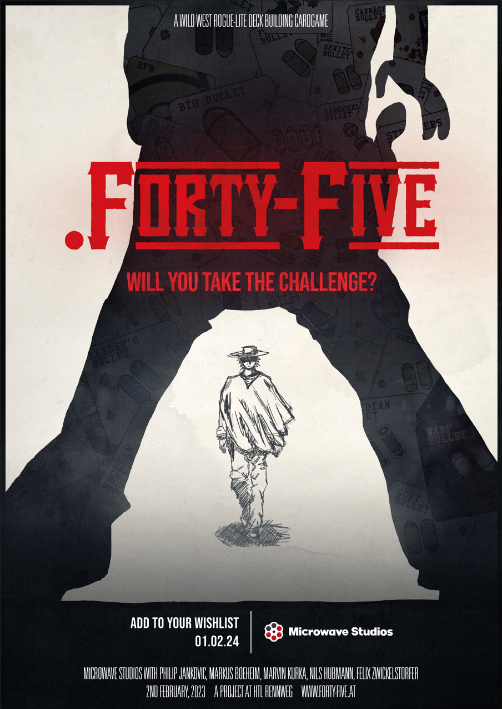
\includegraphics[width=0.7\textwidth]{fortyfivePlakat.png}
    \caption{Das \FF Plakat}
\end{figure}

% resets author
\renewcommand{\kapitelautor}{}
